\documentclass{article}
\usepackage{graphicx}
\begin{document}


Jorge Torres\\
Universidad de Los Andes\\
Metodos Computacionales Taller 5\\
\vspace{1cm}

\begin{figure}[h!]
  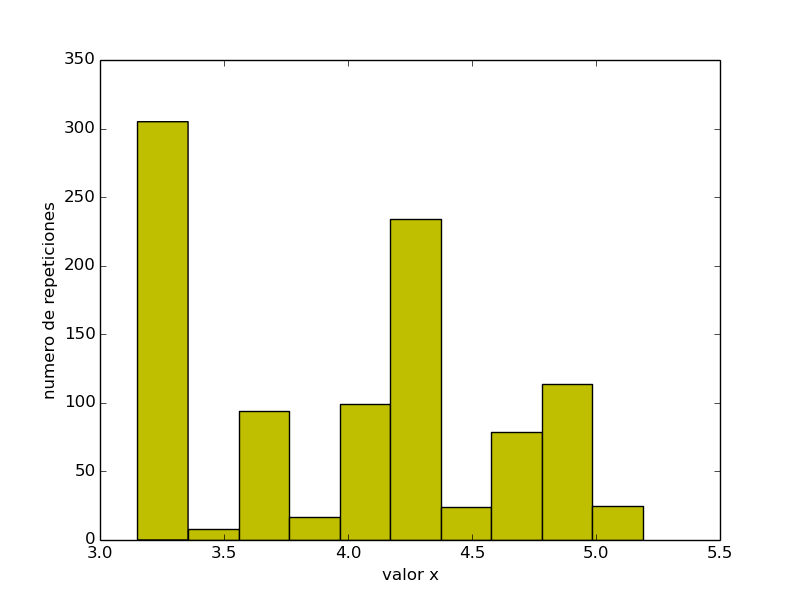
\includegraphics[scale=0.5]{histrogramax.png}
  \caption{Caso 1 Histograma en x }
\end{figure}
Podemos observar que la temperatura de mayor variacion son las condiciones de frontera periodicas, las condiciones fijas convergen a las temperaturas de las paredes del cubo.\\




% git add --all
% git commit -m 'final'
% gir push 

\end{document}